  \documentclass[oneside,a4paper,14pt]{extarticle}
\usepackage[T1,T2A]{fontenc}
\usepackage[a4paper,letterpaper,top=20mm,bottom=20mm,left=30mm,right=10mm]{geometry}
\usepackage{amsmath, amssymb}
\usepackage[utf8]{inputenc}
\usepackage[russian]{babel}
\usepackage{textcomp}
\usepackage{indentfirst}
\usepackage{graphicx}
\usepackage{float}
\usepackage{mwe}
\usepackage{wrapfig} 
\usepackage{caption}
\usepackage{tocloft}
\renewcommand{\cftsecleader}{\cftdotfill{\cftdotsep}}
\usepackage{longtable} 
\usepackage{amsmath}
\usepackage{amsfonts}
\usepackage{amsthm}
\usepackage{float}
\usepackage[all]{xy}
\usepackage[breaklinks]{hyperref}
\usepackage{titlesec}
\usepackage{fancyvrb}

\titleformat{\section}{\normalsize\bfseries}{\thesection}{1em}{}
\titleformat{\subsection}{\normalsize\bfseries}{\thesubsection}{1em}{}
\titleformat{\subsubsection}{\normalsize\bfseries}{\thesubsubsection}{1em}{} 
\captionsetup[figure]{name=Рисунок,labelsep=endash}
\renewcommand\baselinestretch{1.33}\normalsize
\setlength{\parindent}{1.25cm}

\begin{document}
	
	\newpage\thispagestyle{empty}
	\begin{center}
		МИНИСТЕРСТВО НАУКИ И ВЫСШЕГО ОБРАЗОВАНИЯ\\
		РОССИЙСКОЙ ФЕДЕРАЦИИ\\
		ФЕДЕРАЛЬНОЕ ГОСУДАРСТВЕННОЕ БЮДЖЕТНОЕ\\
		ОБРАЗОВАТЕЛЬНОЕ УЧРЕЖДЕНИЕ ВЫСШЕГО ОБРАЗОВАНИЯ\\
		«ВЯТСКИЙ ГОСУДАРСТВЕННЫЙ УНИВЕРСИТЕТ»\\
		Институт математики и информационных систем\\
		Факультет автоматики и вычислительной техники\\
		Кафедра электронных вычислительных машин
	\end{center}
	
	\vspace{20mm}
	\begin{center}
		Отчёт по лабораторной работе №1\\
		по дисциплине\\
		<<Объектно-ориентированное программирование>>\\
	\end{center}
	\vfill
	
	Выполнил студент гр. ИВТб-2301-05-00 \hfill
	\makebox[8cm]{\hrulefill /Ковальский И.И./}
	
	Проверил преподаватель кафедры ЭВМ \hfill
	\makebox[8cm]{\hrulefill /Шмакова Н.А./}
	
	\vfill
	\begin{center}
		Киров\\
		2025
	\end{center}
	
	\newpage
	\setcounter{page}{1}
	\tableofcontents
	\newpage
	
	\section*{Цель работы}
	\addcontentsline{toc}{section}{Цель работы} 
	Освоить на практике начальные этапы жизненного цикла системы согласно стандартам системной инженерии.
	
	\section*{Задание}
	\addcontentsline{toc}{section}{Задание}
	
	\begin{enumerate}
		\item Выбрать тему для разработки
		\item Определить основные функции разрабатываемой системы
		\item Создать прототип пользовательского интерфейса
	\end{enumerate}
	
	\newpage
	
	\section*{Выполнение лабораторной работы}
	\addcontentsline{toc}{section}{Выполнение лабораторной работы}
	
	\subsection*{Выбор темы}
	\addcontentsline{toc}{subsection}{Выбор темы}
	В качестве темы проекта было принято решение выбрать создание онлайн платформы совместного просмотра экранных нарративов. По задумке, сервис предоставляет пользователям возможность создавать группы и добавлять в них других пользователей для дальнейшего совместного просмотра фильмов, с возможностью общения в локальном чате группы.
	
	\subsection*{Основные функции}
	\addcontentsline{toc}{subsection}{Основные функции}
	К основным функциям относятся:
	
	\begin{enumerate}
		\item Регистрация и авторизация пользователей.
		
		\item Поиск фильмов по жанрам.
		
		\item Поиск фильмов по описанию.
		
		\item Возможность оставлять оценки
		
		\item Возможность оставлять комментарии.
		
		\item Возможность совместного просмотра.
		
		\item Возможность общения через чат при совместном просмотре.
	\end{enumerate}
	
	\newpage
	
	\subsection*{Прототип пользовательского интерфейса}
	\addcontentsline{toc}{subsection}{Прототип пользовательского интерфейса}
	
	\begin{figure}[H]
		\centering
		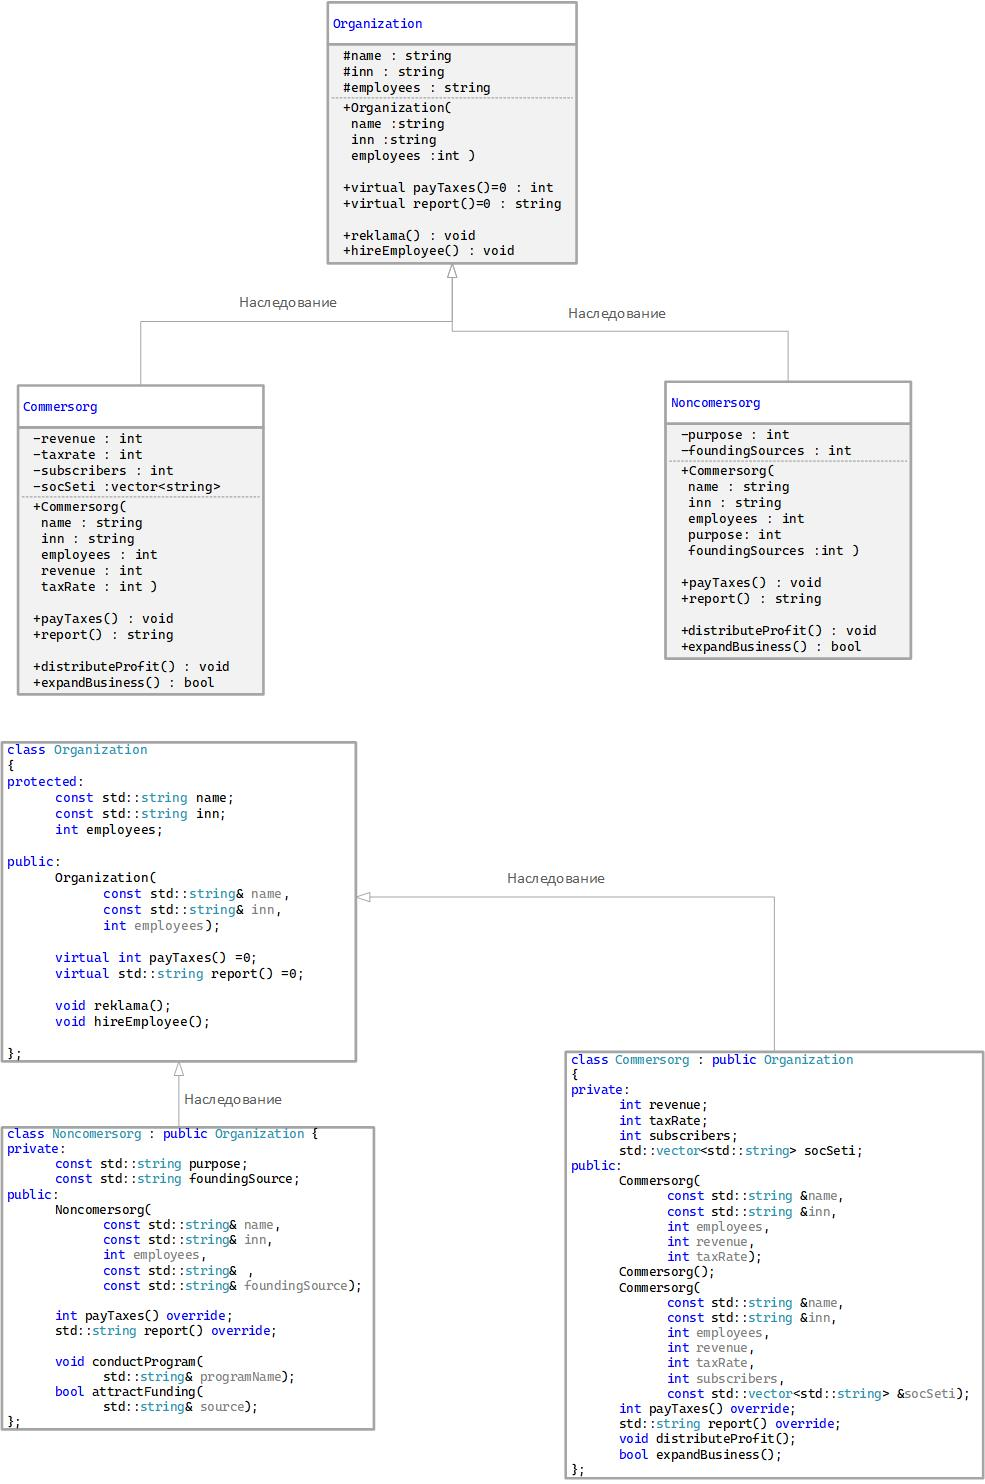
\includegraphics[width=0.9\linewidth]{Диаграмма классов.jpg}
		\caption{Главная страница}
		\label{fig:}
	\end{figure}

	\newpage
	
	\section*{Вывод}
	\addcontentsline{toc}{section}{Вывод}
	В ходе выполнения лабораторной работы было произведено практическое ознакомление с начальными этапами жизненного цикла системы путём выбора темы для проекта, определения его основных функций, создания макета пользовательского интерфейса.
	
\end{document}